% Reconstructed directly from the 1344-line rejected ltl.tex and its PDF,
% using reinvention-outline.md and the live 13-leaf deployment as factual patch.
\documentclass[11pt]{article}
\usepackage[a4paper,margin=1.02in]{geometry}
\usepackage{amsmath,amssymb,amsthm,mathtools}
\usepackage{booktabs,tabularx,array}
\usepackage{enumitem}
\usepackage{xcolor}
\usepackage{lmodern}
\usepackage{microtype}
\usepackage{listings}
\usepackage{tikz}
\usetikzlibrary{arrows.meta,positioning,fit,decorations.pathreplacing,calc}
\usepackage[colorlinks=true,linkcolor=blue!55!black,citecolor=blue!55!black,urlcolor=blue!55!black]{hyperref}
\hypersetup{pdftitle={Accountable Distribution of Machine-Checked Correctness Evidence: A Transparency Model and the Lean Transparency Log},pdfauthor={Olaf Horvath},pdfsubject={Transparency distribution of formal-verification replay evidence},pdfkeywords={formal verification, transparency log, Lean, Ed25519, SLH-DSA, FIPS 205, Merkle tree, attestation}}
\lefthyphenmin=2 \righthyphenmin=3

\newtheorem{definition}{Definition}
\newtheorem{theorem}{Theorem}
\newtheorem{lemma}{Lemma}
\newtheorem{proposition}{Proposition}
\newtheorem{corollary}{Corollary}
\theoremstyle{remark}
\newtheorem{remark}{Remark}

\newcommand{\Hh}{\mathsf{H}}
\newcommand{\hleaf}{\mathsf{h}_{\rm leaf}}
\newcommand{\hnode}{\mathsf{h}_{\rm node}}
\hyphenation{time-stamp time-stamps}
\newcommand{\MTH}{\mathsf{MTH}}
\newcommand{\Root}{\mathsf{Root}}
\newcommand{\Path}{\mathsf{Path}}
\newcommand{\ConsRec}{\mathsf{ConsRec}}
\newcommand{\Obs}{\mathsf{Obs}}
\newcommand{\Policy}{\mathsf{Policy}}
\newcommand{\Fp}{\mathbb{F}_{2^{255}-19}}
\newcommand{\code}[1]{\texttt{\detokenize{#1}}}

\definecolor{deepblue}{RGB}{43,61,112}
\definecolor{deepgreen}{RGB}{28,111,71}
\definecolor{softgray}{RGB}{245,247,249}

\lstset{basicstyle=\ttfamily\small,frame=single,rulecolor=\color{black!15},
backgroundcolor=\color{softgray},columns=fullflexible,keepspaces=true,
showstringspaces=false,breaklines=true,xleftmargin=.5em,xrightmargin=.5em}

\title{\textbf{Accountable Distribution of Machine-Checked Correctness Evidence}\\[3pt]
\large A Transparency Model and the Lean Transparency Log}
\author{Olaf Horvath\\
\small Olaf.Horvath@zkdefi.org \quad ORCID 0009-0004-8008-5805}
\date{July 2026 \\ {\normalsize Revised: August 2026 --- v0.14}}

\begin{document}
\maketitle

\begin{abstract}
Formal verification produces machine-checkable evidence, but consuming that
evidence usually requires the original prover, dependency graph, source
checkout, and substantial replay time. This paper studies a distinct
cryptographic problem: how can a lightweight consumer obtain precise and
accountable assurance about a deterministic proof replay without executing the
verifier and without reducing the result to an opaque provider label?

We define \emph{accountable replay attestation}. A specialized operator performs
an expensive replay once and publishes a structured observation through a
signed append-only log. Consumers verify a signed tree head and logarithmic
inclusion proof, pin history, and apply their own policy to the exact reported axiom-name sets
for each theorem. The construction does not prove that the operator's
observation is true. It makes the claim immutable within a signed view,
comparable across consumers, and attributable when incompatible signed views
are compared.

We instantiate the model as the Lean Transparency Log (LTL), using Lean~4 replay
attestations and an RFC~9162 Merkle tree. We give explicit
collision-extracting arguments for inclusion and consistency, lift them to
scheme-level accountability games with a composition theorem, and evaluate a
live deployment over four production Ed25519 codebases and the verification
path of SLH-DSA (FIPS~205), the hash-based post-quantum signature standard.
The public log contains nineteen leaves, including a Lean mechanization of the
accumulator's own security arguments (61 human-reviewed certificates with one
project-specific uninterpreted SHA-256 boundary axiom) and, as its newest
entry, eleven certificates over the SLH-DSA-SHA2-128s verifier. Since tree
size 14 every signed head additionally carries a deterministic SLH-DSA
co-signature --- produced with the parameter set whose verification path the
log itself attests. The mechanization effort also exposed, via
differential testing, a nontrivial model/implementation divergence --- on
malformed size claims, the deployed iterative consistency verifier was not
extensionally equal to the recursive model proved in Lean (since closed;
this paper reports the pre-closure measurements) --- recorded explicitly
in the corresponding log entry. The contribution is a cryptographic distribution
model for machine-checked correctness evidence, with an end-to-end deployed
instantiation that carries scoped proofs about its own accountability
machinery.
\end{abstract}

\section{Introduction}\label{sec:intro}

Formal verification has made it possible to connect production cryptographic
software to machine-checked mathematics. Systems such as HACL*, EverCrypt,
Fiat-Crypto, and Aeneas demonstrate different routes from implementation to
proof~\cite{hacl,evercrypt,fiatcrypto,aeneas}. Yet the standard assurance story
quietly assumes a capable consumer: one that can retrieve the exact source,
reconstruct the verifier environment, resolve dependencies, and spend minutes
or hours replaying a corpus.

That assumption is often false. A package resolver selecting a cryptographic
backend, a deployment controller enforcing a proof requirement, or an
autonomous custody agent may have milliseconds and a small trusted computing
base, not a theorem prover and thirty minutes of kernel time per candidate.
This creates a problem that is logically downstream of proof construction:

\begin{quote}
\emph{How can a consumer that cannot execute the prover obtain precise,
accountable evidence about a proof replay, without collapsing the result into
an opaque provider verdict?}
\end{quote}

A detached signature on the word ``verified'' authenticates an issuer but does
not bind an ordered history, expose silent replacement, or give consumers a
compact state that can be pinned and required to grow. Shipping the complete
proof and checker preserves direct verification but may defeat the cost and
portability objective. Committees distribute trust but do not themselves fix
the semantics of the attested result. Succinct proofs of verifier execution
would provide validity rather than mere accountability, but require a circuit or
verified-VM representation of the prover and are not yet the deployment
assumption of the artifacts studied here.

We therefore study a narrower primitive: \emph{accountable delegation of
deterministic proof replay}. The operator still observes the replay. The
cryptographic layer does not make that observation true. Instead, it makes the
observation exact, persistent, attributable, and locally policy-checkable.
Independent replay remains the mechanism for challenging a fabricated
observation.

\paragraph{Central thesis.}
The contribution is not a new Merkle tree and not a new theorem prover. It is a
trust decomposition for distributing machine-checked correctness evidence:

\begin{center}
\fbox{\parbox{0.91\linewidth}{\raggedright\hyphenpenalty=10000\exhyphenpenalty=10000
\textbf{Expensive deterministic verification produces an observation.
Transparency makes that observation accountable. Consumer-local policy decides
whether the observation is acceptable.}}}
\end{center}

The Lean Transparency Log (LTL)\footnote{The acronym collides with linear
temporal logic~\cite{pnueli}; we note the collision once and rely on context.}
is the complete instantiation evaluated in this paper. Its subjects are four
Rust Ed25519 codebases with Lean~4~\cite{lean4} certificates against extracted
models. Leaf 12 --- its thirteenth entry --- attests the Lean corpus
that mechanizes the security arguments of the log's own Merkle accumulator
(the tree of \S\ref{sec:construction} together with its inclusion and
consistency verifiers). The paper's central
claim survives replacement of Lean, Ed25519, or RFC~9162 by other components;
what is essential is the distribution and accountability model.

\paragraph{Contributions.}
\begin{enumerate}[leftmargin=1.7em,itemsep=3pt]
\item \textbf{A distribution model for machine-checked evidence.}
We define replay attestations, distinguish observation from verdict, and state
what a lightweight consumer learns without executing Lean.
\item \textbf{A cryptographic accountability layer.}
Using the RFC~9162 tree unchanged, we define signed views, inclusion receipts,
local history pinning, and transferable same-size fork evidence. We give
explicit collision-extracting soundness arguments specialized to the consumer
algorithms, and lift them to scheme level: concrete games for position
binding, history binding, and fork evidence, discharged by explicit
reductions (\S\ref{sec:games}).
\item \textbf{Boundary-conformance policy.}
Each leaf records the exact axiom names reported by Lean. Consumers compare
those observations with their own policy; operator labels can veto but cannot
grant acceptance. We state clearly that axiom-name equality is not semantic
identity of theorem statements.
\item \textbf{A deployed cryptographic case study.}
The log contains nineteen leaves: three replay generations across the four
Ed25519 codebases (the newest at 44 certificates per fork; a \emph{certificate} throughout this paper is one theorem's kernel-checked proof together with its recorded axiom cone), two attestations
of the accumulator's own Lean corpus (leaf 12 carries an environment-derived
audit inventory of 222 compiled constants, 61 human-reviewed certificate
cones, and a single uninterpreted SHA-256 axiom; leaf 17 re-attests the
hardened state), and --- as leaf 18 --- the log's first post-quantum subject:
eleven certificates over the SLH-DSA-SHA2-128s verification path
(Appendix~\ref{app:slhtiers}).
\item \textbf{A negative deployment result.}
Differential testing found that the deployed iterative RFC-style consistency
verifier and the recursive model proved in Lean are not extensionally equal:
there are malformed size/root combinations accepted only by the deployed
verifier. We characterize 3,867 divergences in 73,573 pinned boundary tests
--- every one deployed-accepts-only --- and scope the public attestation
accordingly. (Subsequently closed: the divergence was traced to
the deployed verifier omitting RFC~9162 \S2.1.4.2 Step~7's terminal
$sn=0$ condition; restoring that one conjunct removes every divergence in the
pinned family, confirmed by a three-way regression against an independent
faithful RFC transliteration.)
\end{enumerate}

\paragraph{Non-claims.}
LTL does not prove that the operator honestly reported a kernel run; independent
replay remains the way to detect a fabricated observation. It does not prove
binary correspondence, compiler correctness, extraction faithfulness,
side-channel resistance, SHA-512 correctness, or execution provenance of the
signing binary. The present leaf schema identifies theorem declarations by
repository commit and name, not by a canonical digest of their elaborated Lean
types. These are explicit boundaries, not hidden qualifications
(Appendix~\ref{app:matrix} tabulates every consumer-facing claim with its
establishing mechanism and remaining assumption).

\section{The distribution problem}\label{sec:problem}

\subsection{Three evidence modes}

Let a subject repository at commit $g$ contain theorem declarations
$\Theta_1,\dots,\Theta_q$. A deterministic verifier execution produces an observation
$O_g$ containing success/failure and the reported \emph{axiom cone} (synonymously, the observed axiom-name set) of each
$\Theta_i$ --- the set of axioms the checked proof of $\Theta_i$ ultimately rests on. There are three natural ways to consume this result.

\begin{description}[leftmargin=1.5em,itemsep=4pt]
\item[Direct replay.] The consumer reconstructs the verifier environment and
checks $O_g$ itself. This gives the strongest provenance, but has high
operational cost.
\item[Detached attestation.] A provider signs $O_g$. This is cheap to consume,
but provides no append-only history and no common value for clients to pin.
\item[Transparent attestation.] The provider signs a tree head committing
$O_g$ as one leaf among an ordered history. A consumer verifies inclusion and
persists a head. Incompatible views become attributable when compared.
\end{description}

The third mode is useful precisely when replay is expensive but the result is
stable and deterministic. It does not dominate direct replay: it replaces
local computation with a narrower trust in the replay provider.

\subsection{Why transparency rather than a signature database?}

Suppose an operator signs every replay result independently. Authenticity of
an individual record follows from signature verification, but four properties
are absent:
\begin{enumerate}[leftmargin=1.7em,itemsep=2pt]
\item no signed value commits to the ordered set of all records;
\item the signer commits to no complete ordered history, so omission or
replacement is not detectable by a fresh consumer and carries no compact
consistency proof;
\item two consumers cannot compare a single compact view identifier;
\item a consumer cannot demand that its previously accepted history only grow.
\end{enumerate}
An append-only Merkle tree supplies these missing interfaces. At the current
deployment size, logarithmic proof size is not the decisive benefit;
\emph{history binding} is.

\subsection{Design alternatives}

Table~\ref{tab:alternatives} places the construction among the natural
alternatives, read as a design taxonomy rather than an empirical comparison.
Local replay and proof transport keep semantic checking with the consumer at
high operational cost; detached signatures and committees lower consumer cost
but commit to no ordered history (a committee distributes trust in the
observation; it does not by itself make the record's history accountable);
succinct proofs of replay would upgrade accountability to validity at the
price of proving the prover. LTL occupies the low-consumer-cost point that
still binds an ordered, signed, pinnable history --- and deliberately does not
buy validity of the observation itself.

\begin{table}[t]
\centering\small
\begin{tabularx}{\textwidth}{@{}l>{\raggedright\arraybackslash}X>{\raggedright\arraybackslash}X>{\raggedright\arraybackslash}X>{\raggedright\arraybackslash}X@{}}
\toprule
Mechanism & Consumer cost & Semantic checker & History accountability & Main residual cost \\
\midrule
Local replay & high & consumer & local only & prover/toolchain deployment \\
Proof transport / PCC & medium--high & consumer checker & optional & proof/checker portability \\
Detached signed result & low & provider & statement-level only & replaceable history \\
Committee replay & low & committee & none without an additional log & membership trust \\
Succinct proof of replay & low & circuit/VM verifier & optional & proving the prover \\
LTL & low & provider observes; consumer applies policy & signed append-only views & observation honesty \\
\bottomrule
\end{tabularx}
\caption{Evidence-distribution alternatives. LTL targets low-cost consumers
while retaining an attributable history; it does not remove trust in the
replay observation.}
\label{tab:alternatives}
\end{table}

\section{Model and trust decomposition}\label{sec:model}

\subsection{Roles and objects}

The system has three logical roles.
\begin{description}[leftmargin=1.5em,itemsep=4pt]
\item[Subject maintainer.] Publishes source and proof artifacts at a commit.
\item[Replay operator.] Executes the declared verifier procedure, constructs
an attestation, appends it to the log, and signs tree heads.
\item[Consumer.] Holds the log public key and a local policy; verifies receipts
and optionally persists a previous head.
\end{description}

A replay attestation $a$ contains at least
\[
(\textsf{repo},g,\textsf{toolchain},\textsf{environment},
  [(N_i,s_i,A_i)]_{i=1}^{q}),
\]
where $N_i$ is a declaration name, $s_i$ is replay status, and $A_i$ is the
observed axiom-name set. The deployed schema additionally carries diagnostics,
resource controls, a machine-readable \emph{scope block} (the deployed
leaf-12 instance is quoted verbatim in Appendix~\ref{app:entry13}), and exclusions.

\begin{definition}[Attestation-transparency scheme]
An attestation-transparency scheme is a~\mbox{tuple}
\[
\Pi=(\mathsf{KeyGen},\mathsf{Append},\mathsf{ProveIncl},
\mathsf{VerifyIncl},\mathsf{ProveCons},\mathsf{VerifyCons},\mathsf{Verdict})
\]
over a hash function and signature scheme. $\mathsf{Append}$ commits the
canonical serialization of an attestation as the next leaf and returns a signed
tree head. $\mathsf{Verdict}$ is parameterized by consumer-local policy and
does not consume an operator label as positive evidence.
\end{definition}

\begin{definition}[Accountable replay distribution]
Fix an operator public key and a consumer that persists accepted signed heads.
A replay-distribution scheme is \emph{accountable} if the following hold:
(i) every accepted attestation has an authentic signed view and a uniquely
determined leaf value at its claimed position; (ii) a
consumer accepts a later view only as the same view or a verified extension;
(iii) two valid equal-size heads with unequal roots, in one log and protocol
context, form transferable evidence
that the key holder signed incompatible views, except under signature
forgery; and (iv) positive acceptance of
a theorem boundary is a function of recorded observations and consumer-local
policy, not of an operator label.
\end{definition}

The definition is intentionally an accountability property, not a validity
property. It says when conflicting claims become attributable; it does not
cryptographically prove that the replay observation was honestly produced.
Throughout, ``accountability'' means signed-view and history accountability;
observation validity remains external to the mechanism.
Section~\ref{sec:games} states clauses (i)--(iv) as games and explicit
reductions and proves the construction satisfies them.

\begin{figure}[t]
\centering
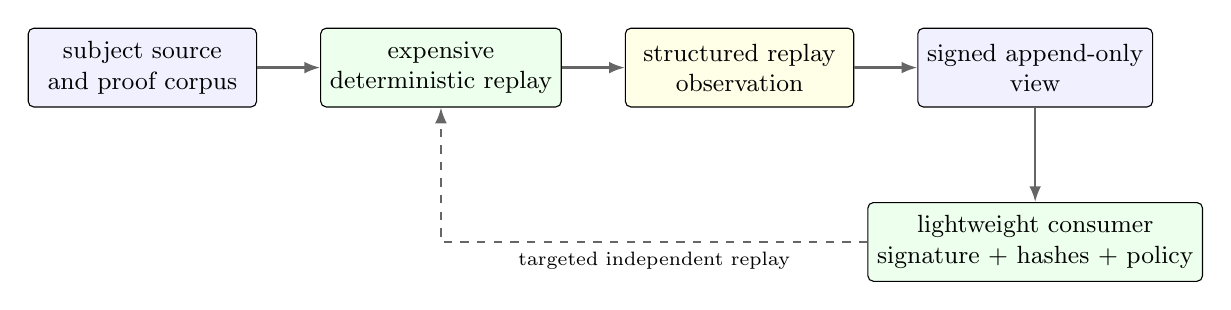
\begin{tikzpicture}[
  node distance=8mm and 8mm,
  b/.style={draw,rounded corners=2pt,align=center,minimum height=10mm,minimum width=29mm,font=\small},
  a/.style={-{Latex[length=2mm]},thick,draw=black!60}
]
\node[b,fill=blue!6] (subject) {subject source\\and proof corpus};
\node[b,fill=green!7,right=of subject] (replay) {expensive\\deterministic replay};
\node[b,fill=yellow!10,right=of replay] (att) {structured replay\\observation};
\node[b,fill=blue!6,right=of att] (log) {signed append-only\\view};
\node[b,fill=green!7,below=12mm of log] (consumer) {lightweight consumer\\signature + hashes + policy};
\draw[a] (subject)--(replay);
\draw[a] (replay)--(att);
\draw[a] (att)--(log);
\draw[a] (log)--(consumer);
\draw[a,dashed] (consumer.west) -| node[pos=.25,below,font=\scriptsize]{targeted independent replay} (replay.south);
\end{tikzpicture}
\caption{Trust decomposition. The log authenticates and orders the replay
operator's observation; it does not replace the theorem prover or make the
observation true.}
\label{fig:decomposition}
\end{figure}

\subsection{What is and is not transferred}

A verified receipt establishes a statement of the form:
\begin{quote}
The holder of public key $pk$ signed a tree head committing, at position $m$,
to a leaf in which the operator reports that the named declarations at commit
$g$ replayed with the recorded axiom-name sets.
\end{quote}
It does not establish that the operator's report is true. Nor does it identify
the semantics of a theorem from its name alone. This separation is central:

\begin{center}\small
\begin{tabular}{@{}ll@{}}
\toprule
Layer & What it contributes \\
\midrule
Lean kernel & validity of a checked term relative to declarations and axioms \\
Replay pipeline & binding of source, toolchain, theorem names, and observations \\
Attestation signature & attribution of one replay statement \\
Merkle log & position binding and append-only view commitments \\
Consumer policy & acceptability of the recorded boundary \\
Independent replay & detection of fabricated operator observations \\
\bottomrule
\end{tabular}
\end{center}

\subsection{Adversary model}

The network adversary may replay, delay, suppress, or substitute messages. The
operator may be malicious: it may construct arbitrary leaves, sign arbitrary
heads, label results arbitrarily, and present different signed views to
different consumers. We assume collision resistance of SHA-256 for the log,
EUF-CMA security of the head-signature scheme, and correct initial acquisition
of the operator public key.

The model deliberately does not cryptographically exclude fabricated kernel
observations; the same holds when the operator's replay harness is defective
rather than dishonest. Whether the kernel actually ran as claimed is a
fact about a physical execution on the operator's machine. The mechanism instead makes the claimed execution target precise
enough for a third party to replay.

\subsection{Consumer goals}

Each goal below is formalized as a game in Section~\ref{sec:games}.

\begin{description}[leftmargin=1.5em,itemsep=5pt]
\item[G1: Authentic position binding.] If a consumer accepts leaf $d$ at
index $m$ under signed head $(n,r)$: the head was issued by the key holder
except under signature forgery, and no leaf distinct from $d$ can also be
opened at position $m$ under that head except under hash collision.
\item[G2: Local append-only history.] A consumer that persists $(n,r)$ accepts
a later view only if it is the same view or a verified extension. Two valid
heads of equal size and unequal roots, in one log context, are transferable
evidence that the key holder signed incompatible views. Unequal-size forks
require retained history, gossip, or a witness. The transition discipline
itself is syntactic, enforced by the pin rule (\S4.3) by construction; the semantic
content --- an opened position cannot change value across accepted views ---
is a theorem (\S\ref{sec:games}).
\item[G3: Policy separation.] The operator's positive label cannot make a
certificate acceptable. The consumer recomputes boundary conformance from
observations and local policy. Operator failure labels may be treated as a
conservative veto.
\end{description}

\subsection{Boundary conformance, not semantic identity}

For certificate $c$, let $\Obs_a(c)$ be the axiom-name set recorded in leaf
$a$, and let $\Policy(c)$ be the consumer's allowed set. Define
\[
\mathsf{boundary\_ok}_a(c) \iff \Obs_a(c)=\Policy(c).
\]
Exact equality detects both additional assumptions and drift in the declared
assurance interface. A missing expected axiom is not automatically a logical
defect: it may indicate a strengthened theorem, a changed statement, a bypassed
abstraction boundary, or stale policy. The consumer therefore rejects or
requires review rather than interpreting the drift.

This predicate is intentionally narrower than ``the intended theorem was
proved.'' The deployed system identifies a declaration by repository commit
and name. A stronger future schema should include canonical digests of the
elaborated theorem type and of the types of declarations in its axiom cone.

\section{Construction}\label{sec:construction}

\subsection{RFC 9162 tree}

Let $\Hh$ be SHA-256. For byte string $d$ and 32-byte values $x,y$ define
\[
\hleaf(d)=\Hh(\mathtt{0x00}\parallel d),\qquad
\hnode(x,y)=\Hh(\mathtt{0x01}\parallel x\parallel y).
\]
For leaf list $D=[d_0,\ldots,d_{n-1}]$:
\[
\MTH([])=\Hh(\epsilon),\qquad \MTH([d])=\hleaf(d),
\]
and for $n>1$,
\[
\MTH(D)=\hnode(\MTH(D[0{:}k]),\MTH(D[k{:}n])),
\]
where $k$ is the largest power of two strictly smaller than $n$. Inclusion and
consistency proofs are the RFC~9162 algorithms~\cite{ct2}.

\subsection{Signed tree heads}

A tree head contains schema-version and type tags, a log identifier, tree
size, root hash, timestamp, and hash-algorithm identifier. The canonical JSON serialization of
those fields is signed with Ed25519. The log identifier and version tag prevent
cross-log and cross-protocol replay. We call the leaf history a head
commits to a \emph{view}, and write \emph{signed view} for that history
as represented by its signed head.

Since tree size 14, every head additionally carries a \emph{deterministic}
SLH-DSA-SHA2-128s (FIPS~205) signature over the same payload. The
co-signature is additive: the Ed25519 signature remains the one every
consumer must verify, and heads published before size 14 carry no
post-quantum signature --- the standalone verifier reports the co-signature as
absent on such heads rather than rejecting them: an append-only log
necessarily preserves the history of its own signature-scheme upgrades. Determinism is chosen as an audit primitive: a
deterministic re-sign of the same payload is byte-comparable, so ``same
input, same signature'' becomes a diff rather than an assurance. The
co-signature closes a further loop: its parameter set is exactly the one
whose verification path is attested at leaf 18
(\S\ref{sec:slhdsa}, Appendix~\ref{app:slhtiers}).

The current implementation records signing-backend provenance alongside the
signature, but that provenance is not execution attestation: an Ed25519
signature does not identify the program that produced it. The public system
therefore treats the claimed signing implementation as operator-reported
context, not as a property proved by the signature.

\subsection{Receipts and pinning}

A receipt contains the leaf index, sibling path, and signed head. A consumer
first verifies the head signature and then reconstructs the root. For history,
a local pin $(n_{\rm pin},r_{\rm pin})$ evolves as follows:
\begin{itemize}[leftmargin=1.6em,itemsep=2pt]
\item same size: accept iff roots match; otherwise retain both signed heads as
same-size fork evidence;
\item larger size: accept iff a consistency proof verifies, then update;
\item smaller size: reject as rollback.
\end{itemize}

We call this transition discipline the \emph{pin rule}, and the persisted
pair $(n_{\mathrm{pin}},r_{\mathrm{pin}})$ the \emph{pin-store}.
Freshness is an external availability policy. A persisted pin detects rollback
relative to local history; it does not prove that a client sees the globally
latest signed head.

\paragraph{Notation summary.}
For reference across the security analysis:

\begin{center}\small
\begin{tabular}{@{}ll@{}}
\toprule
$\Hh$;\ $\hleaf(d)$;\ $\hnode(x,y)$ & SHA-256; leaf hash $\Hh(\mathtt{0x00}\|d)$; node hash $\Hh(\mathtt{0x01}\|x\|y)$ \\
$D$, $d$, $m$, $n$ & leaf list; leaf bytes; leaf index; tree size \\
$\MTH(D)$;\ $k$ & Merkle root; split point (largest power of two below $n$) \\
$\Path(m,D)$;\ $\Root(v,m,n,P)$ & inclusion path (leaf to root); path refold \\
$\mathsf{Open}(d,m,n,P,r)$ & accepting opening: $m<n$ and $\Root(\hleaf(d),m,n,P)=r$ \\
$\ConsRec$;\ $\mathsf{Ext}$ & recursive consistency verifier; pin-rule transition (\S\ref{sec:games}) \\
$C$;\ $b$ & consistency proof; flag: old root is the pinned $r_0$ ($\top$) vs read from $C$ \\
$\Obs_a(c)$;\ $\Policy(c)$ & axiom names recorded in leaf $a$; consumer's allowed set \\
$\chi_{\rm enc}$;\ $\chi=(\chi_{\rm enc},pk)$ & payload-encoded head context; full context with the key \\
$h=(n,r,t;\sigma)$;\ $\mathsf{Vf}_{pk}$ & signed head (size, root, timestamp); signature check \\
$\mathsf{Ev}_\chi$ & same-context, equal-size, unequal-root evidence pair \\
$\mathcal{B}_{\rm pb},\mathcal{B}_{\rm hist},\mathcal{B}_{\rm ha},\mathcal{B}_{\rm fr}$ & the named explicit reductions of \S\ref{sec:games} \\
$Q$;\ $\mathbf{Adv}$ & signing-oracle query set; winning probability (keyed games) \\
\bottomrule
\end{tabular}
\end{center}

\section{Security analysis}\label{sec:security}

This section states the consumer-facing arguments in the form used by the Lean
mechanization. The proofs are elementary but explicit: successful false
openings yield concrete SHA-256 collisions rather than appealing to an informal
``Merkle trees are secure'' statement. The explicitness is load-bearing: over a
fixed-width hash, ``some collision exists'' is trivially true by counting;
each soundness statement therefore names an explicit extractor function,
and the corpus pins a machine-checked guard that each extractor's output
really is a collision (distinct preimages, equal digests).

\subsection{Inclusion}

Let $\Root(v,m,n,P)$ recursively fold value $v$ at position $m$ through proof
path $P$ using the same largest-power-of-two decomposition as $\MTH$. Both
$\Root$ and $\ConsRec$ are partial (the mechanization's \code{Option}):
malformed shapes return a distinguished rejection value, and an equation such
as $\Root(\cdot)=\MTH(D)$ asserts acceptance with that output.

\begin{lemma}[Domain separation]
For all byte strings $d$ and 32-byte values $x,y$,
$\mathtt{0x00}\parallel d \neq \mathtt{0x01}\parallel x\parallel y$.
\end{lemma}
\begin{proof}
The first byte differs.
\end{proof}

\begin{theorem}[Inclusion completeness]
For every non-empty $D$, every $m<|D|$,
\[
\Root(\hleaf(D[m]),m,|D|,\Path(m,D))=\MTH(D).
\]
\end{theorem}
\begin{proof}
By structural induction on $|D|$. The singleton case is immediate. For a split
$D=L\|R$, the honest path is the recursive path inside the side containing $m$
followed by the other side's root. The induction hypothesis reconstructs the
selected child root, and the final node hash reconstructs $\MTH(D)$.
\end{proof}

\begin{theorem}[Inclusion soundness: position binding]
There is an explicit extractor $\mathcal{E}_{\rm incl}$ such that, given $D$,
$m<|D|$, $d\neq D[m]$, and a path $P$ satisfying
\[
\Root(\hleaf(d),m,|D|,P)=\MTH(D),
\]
$\mathcal{E}_{\rm incl}(D,m,d,P)$ returns two distinct SHA-256 preimages with
the same digest.
\end{theorem}
\begin{proof}
Recompute the honest tree and replay the accepting reconstruction from the root
downward. At each visited internal node, compare the adversarial and honest
node preimages. If they differ while their digests agree, output the collision.
Otherwise both child values agree and descent continues along the path. At the
terminal leaf, equality of digests with $d\neq D[m]$ yields a leaf-hash
collision. Domain separation rules out interpreting a leaf preimage as a node
preimage without already producing a collision.
\end{proof}

\subsection{Consistency}

The recursive verifier $\ConsRec(n_0,n_1,C,b,r_0)$ reconstructs an old and new
root from proof $C$, a flag $b$ indicating whether the old root is implicit,
and pinned value $r_0$. Malformed shapes return rejection.

\begin{theorem}[Consistency soundness of the recursive model]
There is an explicit extractor $\mathcal{E}_{\rm cons}$ such that, whenever
$|D_0|=n_0\le n_1=|D_1|$, $D_0\neq D_1[0{:}n_0]$, and
\[
\ConsRec(n_0,n_1,C,\top,\MTH(D_0))
   =(\MTH(D_0),\MTH(D_1)),
\]
$\mathcal{E}_{\rm cons}(D_0,D_1,C)$ returns a SHA-256 collision. (The hypothesis supplies the honest
$\MTH(D_0)$ as the pinned value; \S5.3 measures the deployed flow, which
has no such mechanized supplier.)
\end{theorem}
\begin{proof}
The new-root component is a hash fold over the shape of the $n_1$ tree. Compare
it with the honest $D_1$ tree. Either the first differing preimage gives a
collision, or every consumed proof node equals the corresponding honest node.
In the latter case, the old-root component is the canonical fold of the honest
prefix $D_1[0{:}n_0]$, so acceptance implies
$\MTH(D_0)=\MTH(D_1[0{:}n_0])$. The two equal-sized leaf lists differ; descend
through their identically shaped honest trees to extract the first hash
collision.
\end{proof}

The theorem's hypothesis pins the honest old root $\MTH(D_0)$. The deployed
flow contains nothing mechanized that guarantees the pinned value is the
honest old root; the next subsection measures the iterative verifier's
behavior when only the claimed sizes constrain its reconstruction.

\begin{proposition}[Pin-store safety]
Assume EUF-CMA security of the head signature and collision resistance of
SHA-256. A consumer following the pin transition accepts only a nondecreasing
sequence of sizes; if leaf lists are exhibited for two accepted heads,
they are prefix-related except under collision (see the mapping paragraph
of \S\ref{sec:games}). Two accepted
heads under the same key, in one log context, with equal size and unequal
roots are transferable evidence that the key holder signed incompatible
views.
\end{proposition}
\begin{proof}
Rollback is rejected syntactically. At equal size the transition is accepted
only with equal roots; if the two exhibited equal-length leaf lists differed,
whole-tree root binding (each root determines its committed leaf list up
to collision) would extract a SHA-256 collision, so under collision
resistance the lists are equal. A larger head is accepted only after a
consistency proof, so non-prefix acceptance yields a collision by the previous
theorem. Equal-size unequal roots in one log context, with valid signatures, are two
conflicting statements attributable to the key holder, except under signature
forgery.
\end{proof}

\begin{proposition}[Policy separation]
For fixed local policy $\Policy$, the boundary-conformance result for every
certificate is a function only of $\Obs_a(c)$ and $\Policy(c)$. An operator
label cannot change a nonconforming observation into a conforming one.
\end{proposition}
\begin{proof}
The comparison is set equality and takes no positive operator label as input.
A deployment may conservatively treat an operator failure label as a veto, but
a veto cannot grant acceptance.
\end{proof}

\subsection{Scope of the deployed consistency claim}\label{sec:seamscope}

The Lean theorem covers the recursive predicate above. The deployed iterative
verifier follows the familiar RFC bit-navigation algorithm. Differential
testing discovered that the two verifiers are not extensionally equal on
malformed size claims, every observed divergence being accepted only by the
iterative verifier: for example, a valid proof for a $2\to3$ transition can
be accepted under the false old-size claim $1\to3$ when paired with the size-2
root. The mechanism is elementary: the iterative algorithm seeds its
reconstruction with the supplied old root and consults the size claims only as
bit-navigation state, so several distinct old-size claims navigate one proof
identically. In 73,573 lied-size boundary cases, 3,867 divergences were
observed; all were one-sided (deployed accepts, recursive model rejects).
The root cause was later identified and closed: the deployed loop omitted
RFC~9162 \S2.1.4.2 Step~7's terminal $sn=0$ condition; with the conjunct
restored the pinned family shows zero divergences (three-way regression:
deployed verifier, recursive model, independent RFC transliteration).

The intended consumer flow binds $(n_0,r_0)$ in local persistent state and
binds $(n_1,r_1)$ together in a signed head. The present corpus does not prove
a refinement theorem from that operational invariant to the recursive
predicate. Consequently the public attestation says exactly this: the model is
proved; deployment correspondence is finite-tested and relies on an
unmechanized authentic-size/root invariant.

\subsection{Scheme-level games and a composition theorem}\label{sec:games}

The theorems above bind single artifacts to a reference leaf list. This
subsection lifts them to the scheme. Readers content with the component
theorems can skim the statements --- the four games,
Definition~\ref{def:formal}, Theorem~\ref{thm:main} --- and the closing
mapping paragraph; the proofs add explicit reductions but no new assumptions.

Fix once, for the entire subsection, an \emph{encoded context}
\[\chi_{\rm enc}=(\text{log identifier},\ \text{schema and type tags},\
\text{hash-algorithm identifier});\]
every head below is required to encode $\chi_{\rm enc}$ in its canonical
payload, matching the deployed head format of \S4.2. The verification key is
deliberately \emph{not} part of the payload: it is the external verification
parameter, and we write $\chi=(\chi_{\rm enc},pk)$ for the full context once
a key exists --- the keyed games fix $\chi_{\rm enc}$, run
$\mathsf{KeyGen}$, and then set $\chi$.

The results come in two levels. The theorems are unconditional: explicit
algorithms turn any winning transcript into a concrete SHA-256 collision,
and the signature reductions lose exactly one EUF-CMA forgery. Hardness
enters only at the end: SHA-256 is a fixed, unkeyed function, so following
the human-ignorance treatment~\cite{rogaway}, Corollary~\ref{cor:security}
states the constructive consequence --- an explicit winner yields an explicit
collision finder --- and labels the security reading as the engineering
judgment it is. (A keyed-family restatement is routine and omitted.)

The position-binding and history games are non-interactive: they are
universal statements over accepted transcripts, independent of how a
transcript was obtained, so adaptive interaction with a proof-issuing
service collapses into the adversary's final output. Signatures constrain
two other parties --- an outsider forging an ordinary head
($\mathsf{HEAD}$), and a third party fabricating equivocation evidence
($\mathsf{FORK}$); those games have a secret and a signing oracle, and their
advantage is the probability, over key generation and the adversary's coins,
of winning. The adversary may query the signing oracle adaptively on
context-valid payloads; $Q$ denotes the set of exact queried payload bytes.

\paragraph{The games at a glance.}
\begin{center}\footnotesize
\begin{tabular}{@{}lllll@{}}
\toprule
Game & Adversary & Secrets & Wins by exhibiting & Consequence \\
\midrule
$\mathsf{PB}$ & operator (holds key) & none & two openings, one position, $d\neq d'$ & collision (Thm.~\ref{thm:pb}) \\
$\mathsf{HIST}$ & operator & none & accepted chain, changed opened value & collision (Thm.~\ref{thm:hist}) \\
$\mathsf{HEAD}$ & outsider & signing oracle & valid head never issued & forgery (Thm.~\ref{thm:head}) \\
$\mathsf{FORK}$ & third party & signing oracle & evidence pair not fully issued & forgery (Thm.~\ref{thm:fork}) \\
\bottomrule
\end{tabular}
\end{center}
\noindent Policy separation is deliberately not a game: it is a deterministic
property of the verdict algorithm (Lemma~\ref{lem:policy}).

\paragraph{Accepted-artifact syntax.}
A head is $h=(n,r,t;\sigma)$, with $t$ a timestamp; its canonical payload is
$\mathsf{EncodeHead}_{\chi_{\rm enc}}(n,r,t)$ as in \S4.2, and $\mathsf{Vf}_{pk}(h)=1$
iff its Ed25519 signature verifies. An \emph{opening}
of leaf $d$ at index $m$ under $(n,r)$ is a path $P$ with $m<n$ and
$\Root(\hleaf(d),m,n,P)=r$ (acceptance in the Option sense of \S5.1); write
$\mathsf{Open}(d,m,n,P,r)=1$. An \emph{extension} from $(n_0,r_0)$ to
$(n_1,r_1)$ by proof $C$ is exactly a pin-rule transition: either $n_0=n_1$,
$r_0=r_1$, and $C$ is empty, or $n_0<n_1$ and
$\ConsRec(n_0,n_1,C,\top,r_0)=(r_0,r_1)$; write
$\mathsf{Ext}(n_0,r_0,n_1,r_1,C)=1$.

\begin{lemma}[Monotone extensions]\label{lem:mono}
If $\mathsf{Ext}(n_0,r_0,n_1,r_1,C)=1$ then $n_0\le n_1$; accepted chains of
extensions have nondecreasing sizes.
\end{lemma}
\begin{proof}
Immediate from the two disjuncts of $\mathsf{Ext}$.
\end{proof}

\begin{lemma}[Payload injectivity]\label{lem:inj}
For fixed $\chi_{\rm enc}$, $\mathsf{EncodeHead}_{\chi_{\rm enc}}$ is
injective on $(n,r,t)$; in particular, distinct $(n,r)$ pairs yield distinct
payload byte strings.
\end{lemma}
\begin{proof}
The canonical serialization emits a fixed set of keys in sorted order with
fixed separators; the size is a decimal integer, the root a fixed-length
lowercase hex string, and the timestamp a JSON string with injective
escaping, all under distinct fixed keys, so the encoding parses back
uniquely. This is injectivity of the specified serializer over the restricted
head schema, not a claim about arbitrary JSON.
\end{proof}

\paragraph{Game $\mathsf{PB}$ (position binding).}
$\mathcal{A}$ outputs $(n,r,m,d,P,d',P')$ and wins iff $d\neq d'$ and
\[\mathsf{Open}(d,m,n,P,r)=\mathsf{Open}(d',m,n,P',r)=1.\]

\begin{theorem}[Scheme position binding]\label{thm:pb}
There is an explicit algorithm $\mathcal{B}_{\rm pb}$ that, whenever
$\mathcal{A}$ wins $\mathsf{PB}$, outputs two distinct byte strings with
equal SHA-256 digests, using at most the $2(\lceil\log_2 n\rceil{+}1)$ hash
evaluations of replaying the two openings, with their intermediate values
retained.
\end{theorem}
\begin{proof}
Both accepting folds have the shape determined by $(m,n)$ and output the same
root $r$. Walk from the root downward along the path of $m$, maintaining that
the two transcripts agree on the current node's value. At an internal node
the transcripts present preimages $\mathtt{0x01}\|a\|b$ and
$\mathtt{0x01}\|a'\|b'$ with equal digests; since child values have fixed
32-byte width, the argument pairs are recoverable from the preimages, so
unequal pairs are a collision and equal pairs propagate agreement one level
down. If no disagreement occurs, the leaf presents $\mathtt{0x00}\|d$ and
$\mathtt{0x00}\|d'$ with equal digests and $d\neq d'$ --- a collision. Since
the shapes coincide, every comparison is leaf-to-leaf or node-to-node; domain
separation would in addition make any cross-type coincidence itself a
collision of distinct strings.
\end{proof}

\paragraph{The transport algorithm.}
For the history theorem we need to move an opening backward through an
accepted extension. Recall the recursive verifiers (\S4.1, the mechanized
form; malformed shapes reject); Figure~\ref{fig:transport} shows the assembly in a
small instance. With $k$ the largest power of two below $n$:
\[
\Root(v,m,n,P)=
\begin{cases}
v & n=1,\ P\ \text{exhausted}\\
\hnode(\Root(v,m,k,P'),\,s) & m<k\\
\hnode(s,\,\Root(v,m{-}k,n{-}k,P')) & m\ge k,
\end{cases}
\]
where $s$ is the sibling $P$ supplies for the current level, and
\[
\ConsRec(n_0,n,C,b,r)=
\begin{cases}
(v,v),\ \ v=r\ \text{if}\ b\ \text{else the next value of}\ C & n_0=n\\
(x,\ \hnode(y,s)) & n_0\le k\\
(\hnode(s,x),\ \hnode(s,y)) & n_0>k,
\end{cases}
\]
where in the second branch $(x,y)=\ConsRec(n_0,k,C,b,r)$ and $s$ is the next
value of $C$, and in the third branch $s$ is the next value of $C$ and
$(x,y)=\ConsRec(n_0{-}k,n{-}k,C,\bot,r)$. Both recursions' shapes are
determined by their integer arguments, not by the adversary, so two
computations at the same arguments traverse the same nodes and there are no
mismatched stopping points.

\begin{figure}[htbp]
\centering
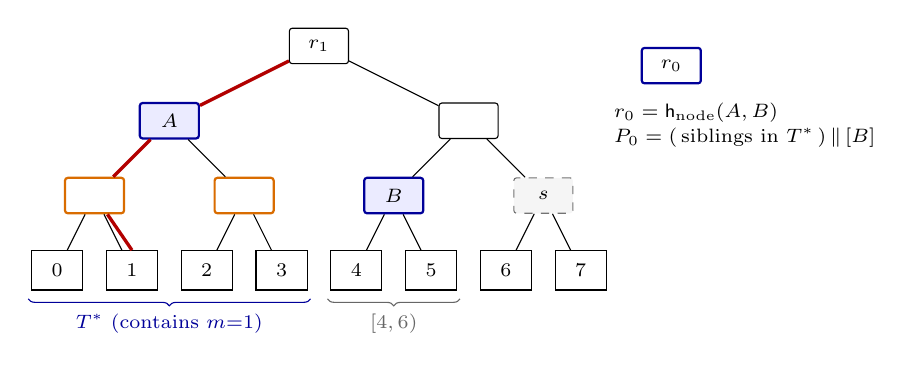
\begin{tikzpicture}[
  every node/.style={font=\scriptsize},
  lf/.style={draw,minimum width=6.5mm,minimum height=5mm,inner sep=1pt},
  nd/.style={draw,rounded corners=1pt,minimum width=7.5mm,minimum height=4.5mm,inner sep=1pt,fill=white},
  fr/.style={nd,draw=blue!60!black,thick,fill=blue!8},
  pn/.style={nd,draw=black!55,dashed,fill=black!4},
  sb/.style={draw=orange!85!black,thick},
  op/.style={draw=red!70!black,very thick}
]
\foreach \i in {0,...,7} \node[lf] (d\i) at (0.95*\i,0) {$\i$};
\node[nd,sb] (p01) at (0.475,0.95) {};
\node[nd,sb] (p23) at (2.375,0.95) {};
\node[fr] (p45) at (4.275,0.95) {$B$};
\node[pn] (p67) at (6.175,0.95) {$s$};
\node[fr] (q03) at (1.425,1.9) {$A$};
\node[nd] (q47) at (5.225,1.9) {};
\node[nd] (rt) at (3.325,2.85) {$r_1$};
\foreach \a/\b in {d0/p01,d1/p01,d2/p23,d3/p23,d4/p45,d5/p45,d6/p67,d7/p67,p01/q03,p23/q03,p45/q47,p67/q47,q03/rt,q47/rt}
  \draw (\a) -- (\b);
\draw[op] (d1.north) -- (p01); \draw[op] (p01) -- (q03); \draw[op] (q03) -- (rt);
\draw[decorate,decoration={brace,mirror,raise=3pt},blue!60!black]
  ([xshift=-1pt]d0.south west) -- ([xshift=1pt]d3.south east)
  node[midway,below=5pt]{$T^*$ (contains $m{=}1$)};
\draw[decorate,decoration={brace,mirror,raise=3pt},black!60]
  ([xshift=-1pt]d4.south west) -- ([xshift=1pt]d5.south east)
  node[midway,below=5pt]{$[4,6)$};
\node[nd,draw=blue!60!black,thick] (r0) at (7.8,2.6) {$r_0$};
\node[align=left,anchor=north west] at (6.95,2.25)
  {$r_0=\hnode(A,B)$\\[1pt]$P_0=(\,\text{siblings in }T^*\,)\,\|\,[B]$};
\end{tikzpicture}
\caption{Prefix transport in the $6\to8$ instance, opening at index $m=1$.
The accepted consistency transcript pins the frontier values $A,B$ covering
$[0,6)$ (solid blue) and consumes the proof value $s$ covering $[6,8)$
(dashed). Comparing the opening's fold (red path) with the transcript fixes
the opening's value at the frontier subtree $T^*$ containing $m$. Below
$T^*$ the opening keeps its own siblings (orange); above it, the old-root
fold $r_0=\hnode(A,B)$ supplies the one remaining sibling $B$. The assembled
$P_0$ is the opening's inner path with the new tree's top sibling replaced
by $B$.}
\label{fig:transport}
\end{figure}


\begin{samepage}
\begin{lemma}[Prefix transport]\label{lem:transport}
Suppose $m<n_0\le n_1$ and
\[\mathsf{Ext}(n_0,r_0,n_1,r_1,C)=1, \qquad \mathsf{Open}(d,m,n_1,P,r_1)=1.\]
There is an explicit algorithm $\mathsf{Transport}$ returning either two
distinct byte strings with equal SHA-256 digests, or a path $P_0$ with
$\mathsf{Open}(d,m,n_0,P_0,r_0)=1$, using at most the hash evaluations of
replaying the two accepted transcripts.
\end{lemma}
\end{samepage}
\begin{proof}
If $n_0=n_1$ then $r_0=r_1$ and $P_0=P$. Otherwise
$\ConsRec(n_0,n_1,C,\top,r_0)=(r_0,r_1)$, and we prove the following claim by
strong induction on $n$ --- both sub-calls strictly decrease it --- for every
sub-call arising in the accepted transcript:

\emph{Claim.} If $\ConsRec(n_0',n,C',b,\cdot)$ accepts with output $(x,y)$,
and $\mathsf{Open}(d,m',n,P',\rho)=1$ with $m'<n_0'$ and $\rho=y$, then
either an explicit collision is output, or a path $P_0'$ with
$\mathsf{Open}(d,m',n_0',P_0',x)=1$.

\emph{Base} ($n_0'=n$): the transcript gives $x=y=\rho$, and $P_0'=P'$.

\emph{Case} $n_0'\le k$, $k$ the split of $n$: the transcript's second
component is $y=\hnode(y_L,s)$ with $(x,y_L)$ the left sub-call's output.
Since $m'<n_0'\le k$, the opening's top step is
$\rho=\hnode(u,s_P)$ with $u=\Root(\hleaf(d),m',k,\cdot)$ accepted on the
opening's remaining path. The two preimages of $\rho=y$ are
$\mathtt{0x01}\|y_L\|s$ and $\mathtt{0x01}\|u\|s_P$: if the pairs differ,
output the collision; otherwise $u=y_L$, and the inductive hypothesis applied
to the left sub-call (output $(x,y_L)$) and the sub-opening (root value
$u=y_L$) yields a collision or $P_0'$ with
$\mathsf{Open}(d,m',n_0',P_0',x)=1$, which is the claim since the first
component passes through this branch unchanged.

\emph{Case} $n_0'>k$: the transcript consumed $s$ and the right sub-call
returned $(x_R,y_R)$, so $x=\hnode(s,x_R)$ and $y=\hnode(s,y_R)$. Because
$k<n_0'\le n$ and $k$ is the largest power of two below $n$, $k$ is also the
largest power of two below $n_0'$ (there is no power of two strictly between
$k$ and $n$; mechanized in the corpus as \code{kbelow_prefix_eq}), so the $n_0'$-tree splits at $k$ as well and
$x=\hnode(s,x_R)$ is precisely its root form.
\emph{If} $m'<k$: the opening's top step is $\rho=\hnode(u,s_P)$ with
$u=\Root(\hleaf(d),m',k,\cdot)$ accepted on the remaining path
$P'_{\rm in}$. Compare preimages of $\rho=y$: unequal pairs are a collision;
otherwise $u=s$ and $s_P=y_R$, so the remaining path opens $d$ at $m'$ in the
left subtree with root value $s$, and
$P_0'\coloneqq P'_{\rm in}\,\|\,[x_R]$ satisfies
$\Root(\hleaf(d),m',n_0',P_0')=\hnode(s,x_R)=x$: an accepting opening,
assembled from the opening's own inner path and the transcript's right
first-component. \emph{If} $m'\ge k$: the opening's top step is
$\rho=\hnode(s_P,u)$ with $u$ accepted at $m'-k$ in the right subtree;
comparing preimages of $\rho=y$ either yields a collision or $s_P=s$ and
$u=y_R$, and the inductive hypothesis on the right sub-call (output
$(x_R,y_R)$, sizes $n_0'-k\le n-k$, index $m'-k<n_0'-k$) gives a collision or
$P_0''$ opening $d$ at $m'-k$ under $x_R$; then
$P_0'\coloneqq P_0''\,\|\,[s]$ opens $d$ at $m'$ under $x=\hnode(s,x_R)$.

The top-level instance of the claim has $\rho=r_1=y$ and $x=r_0$ by
acceptance, which is the lemma. Every comparison is between two explicit
32-byte-child node preimages, so each disagreement is a concrete collision;
every assembled path entry is either an entry of $P$, an entry of $C$, or a
sub-call output value, all present in the replayed transcripts.
\end{proof}

In the smallest growth case $2\to3$ --- the log's own transition in
\S\ref{sec:seamscope} --- $n_0$ is a power of two: the frontier is the whole
old tree and $P_0$ is simply the opening's within-prefix tail.

\paragraph{Game $\mathsf{HIST}$ (local history binding).}
$\mathcal{A}$ outputs a chain of head values $h_0,\dots,h_\ell$, transition
proofs $C_1,\dots,C_\ell$ with $\mathsf{Ext}(n_{i-1},r_{i-1},n_i,r_i,C_i)=1$
for every $1\le i\le \ell$, indices $0\le a<b\le \ell$, an index $m<n_a$, and
openings with
$\mathsf{Open}(d,m,n_a,P,r_a)=\mathsf{Open}(d',m,n_b,P',r_b)=1$ and
$d\neq d'$. $\mathcal{A}$ wins iff everything verifies. (The chain is the
Merkle-level state sequence a consumer's pin traverses; authentication is
$\mathsf{HEAD}$'s job, and the binding properties quantify over accepted
transcripts regardless of provenance.)

\begin{theorem}[History binding]\label{thm:hist}
There is an explicit algorithm $\mathcal{B}_{\rm hist}$ that, whenever
$\mathcal{A}$ wins $\mathsf{HIST}$, outputs a SHA-256 collision, using
$O(\ell\log n_\ell)$ hash evaluations.
\end{theorem}
\begin{proof}
By Lemma~\ref{lem:mono}, $m<n_a\le n_i$ for all $i\ge a$. Walk $t$ from $b$
down to $a{+}1$, maintaining an accepting opening of $d'$ at $m$ under
$(n_t,r_t)$. If $n_{t-1}=n_t$ then $\mathsf{Ext}$ forces $r_{t-1}=r_t$ and
the opening carries over unchanged; if $n_{t-1}<n_t$, apply
Lemma~\ref{lem:transport} to $C_t$ and the current opening, obtaining a
collision (done) or an accepting opening under $(n_{t-1},r_{t-1})$. Arriving
at $h_a$ yields two accepting openings of $d\neq d'$ at $m$ under
$(n_a,r_a)$, and Theorem~\ref{thm:pb} extracts the collision. Accepted
transcripts have their RFC-determined logarithmic length --- malformed
lengths reject --- so the walk costs at most the evaluations of replaying the
$\ell$ transition transcripts and the two openings.
\end{proof}

\paragraph{Game $\mathsf{HEAD}$ (head authenticity).}
A challenger runs $\mathsf{KeyGen}$ and signs, on the operator's behalf, the
canonical payloads the operator issues in context $\chi_{\rm enc}$ (query
set $Q$). The adversary, without the key, outputs a head $h$ and wins iff
$\mathsf{Vf}_{pk}(h)=1$, $h$ encodes $\chi_{\rm enc}$, and $h$'s payload is
not in $Q$.

\begin{theorem}[Head authenticity]\label{thm:head}
For every $\mathcal{A}$ there is an explicit $\mathcal{B}_{\rm ha}$ with
$\mathbf{Adv}^{\mathsf{HEAD}}(\mathcal{A})\le
\mathbf{Adv}^{\text{euf-cma}}(\mathcal{B}_{\rm ha})$: a winning head's exact
payload bytes were never queried, so its valid signature is an existential
forgery, which $\mathcal{B}_{\rm ha}$ outputs.
\end{theorem}

\paragraph{Game $\mathsf{FORK}$ (fork evidence).}
Define the context-scoped evidence predicate:
$\mathsf{Ev}_\chi(h,h')=1$ iff both signatures verify under $pk$, both heads
encode the same $\chi_{\rm enc}$, the tree sizes are equal, and the roots
differ. Heads of
different logs, schema versions, or hash algorithms never form evidence ---
one key legitimately operating two logs must not be classifiable as
equivocating. \emph{Completeness} is by construction: if the key holder signs
two equal-size, unequal-root heads in one context, the pair itself satisfies
$\mathsf{Ev}_\chi$; producing it requires retention and comparison, not
cooperation. \emph{Frame resistance} is the game: the challenger signs the
operator's issued payloads in $\chi_{\rm enc}$ (query set $Q$); the
adversary, without the key, outputs $(h,h')$ and wins iff $\mathsf{Ev}_\chi(h,h')=1$ and at
least one of the two payloads is not in $Q$. This is an
\emph{issued-message attribution} game: a valid evidence pair proves the key
holder signed both conflicting payloads, except with forgery probability.

\begin{theorem}[Frame resistance]\label{thm:fork}
For every $\mathcal{A}$ there is an explicit $\mathcal{B}_{\rm fr}$ with
$\mathbf{Adv}^{\mathsf{FORK}}(\mathcal{A})\le
\mathbf{Adv}^{\text{euf-cma}}(\mathcal{B}_{\rm fr})$.
\end{theorem}
\begin{proof}
A winning pair contains a head whose exact canonical payload bytes were never
queried to the signing oracle; its valid signature is an existential forgery,
which $\mathcal{B}_{\rm fr}$ outputs.
\end{proof}

\begin{lemma}[Policy separation --- Proposition~2 restated for the scheme package]\label{lem:policy}
For every leaf $a$ and certificate $c$, the verdict computed by
$\mathsf{Verdict}$ equals $[\Obs_a(c)=\Policy(c)]$; it reads no operator
label, and acceptance consults the operator's status only as a veto. This is
a deterministic property of the $\mathsf{Verdict}$ algorithm, by construction
(\S\ref{sec:model}); it is not a hardness statement.
\end{lemma}

\begin{definition}[Collision-extractable accountability]\label{def:formal}
A scheme with fixed context $\chi$ is \emph{collision-extractably
accountable} if there are explicit algorithms, running in time polynomial in
the transcript size, that map every winning $\mathsf{PB}$ or $\mathsf{HIST}$
output to two distinct strings with equal hash digests; explicit reductions
bounding $\mathbf{Adv}^{\mathsf{HEAD}}$ and $\mathbf{Adv}^{\mathsf{FORK}}$
each by one EUF-CMA advantage; and a $\mathsf{Verdict}$ satisfying policy
separation.
\end{definition}

\begin{theorem}[Collision-extractable accountability of the construction]\label{thm:main}
The LTL construction with the recursive verifiers of \S\ref{sec:security}
--- the RFC~9162 tree, the canonical signed heads of \S4.2 in their fixed context $\chi$, the pin rule of \S4.3, and the policy
verdict of \S\ref{sec:model} --- is collision-extractably accountable, with
$\mathcal{B}_{\rm pb}$ ($\le 2(\lceil\log_2 n\rceil{+}1)$ hash evaluations),
$\mathcal{B}_{\rm hist}$ ($O(\ell\log n_\ell)$), and the one-forgery reductions
$\mathcal{B}_{\rm ha},\mathcal{B}_{\rm fr}$ of
Theorems~\ref{thm:pb}--\ref{thm:fork}.
\end{theorem}

\begin{corollary}[Constructive security consequence]\label{cor:security}
For every explicitly given feasible adversary that wins $\mathsf{PB}$ or
$\mathsf{HIST}$, the explicitly specified $\mathcal{B}_{\rm pb}$ and
$\mathcal{B}_{\rm hist}$ constitute an explicitly given SHA-256 collision
finder, feasible with the explicit overhead stated in
Theorems~\ref{thm:pb} and~\ref{thm:hist}. For every explicitly given
feasible $\mathsf{HEAD}$ or $\mathsf{FORK}$ adversary, the stated black-box
reductions give an Ed25519 EUF-CMA forger with no loss in success
probability, under correct initial acquisition of $pk$ and the fixed context.
Under the human-ignorance reading of collision resistance~\cite{rogaway} ---
no feasible SHA-256 collision finder is presently known --- this yields the
intended security interpretation; that reading is an engineering judgment
stated as such, not a mathematical assumption discharged by this corollary.
\end{corollary}

\paragraph{What the games do and do not formalize.}
Against Definition~2: clause (i) is delivered as head authenticity
($\mathsf{HEAD}$) plus opening \emph{uniqueness} ($\mathsf{PB}$) --- no
distinct leaf can also be opened at an accepted position. Whether a root
moreover commits a complete published leaf list is a system property, not a
game property: the log publishes its leaves, and a consumer holding the
mirror checks membership against the actual list. In short,
$\mathsf{PB}$ proves leaf-value binding; mirror recomputation proves
equality to the published list. Clause (ii) splits into a
syntactic part --- the pin rule accepts only same-view or verified-extension
transitions, by construction --- and the semantic part supplied by
$\mathsf{HIST}$: a position opened in two accepted views cannot change value
without a collision. Clause (iii) is $\mathsf{FORK}$ completeness and frame
resistance, scoped to $\chi$. Clause (iv) is Lemma~\ref{lem:policy}. The games adapt the established
two-transcript secure-logging notions~\cite{dghs} to replay attestation ---
operator as first-class adversary, policy separation added.

\begin{remark}[What is mechanized, what is not]\label{rem:gamescope}
The games are stated for the scheme's specified verifiers --- the recursive
model whose honest-reference specializations are kernel-checked in leaf~12
(the named extractors and per-step pin safety). The two-transcript
comparisons and the transport induction are paper-level proofs in the same
discipline --- the induction reuses the corpus's mechanized
\code{kbelow_prefix_eq} fact --- and are not part of the mechanized corpus;
$\mathsf{HIST}$ supplies, at paper level, the multi-step closure the corpus
leaves external. Applying any of these statements to the deployed iterative
verifier inherits the refinement boundary of the previous subsection
unchanged.
\end{remark}

\section{Lean instantiation: Ed25519 and SLH-DSA}\label{sec:instantiation}

\subsection{Proof corpus}

The initial subjects are upstream \code{curve25519-dalek}/\code{ed25519-dalek}
(one implementation: the curve crate and the signature crate atop it) and
three deployed forks: Solana/Anza, RISC~Zero, and Betrusted --- all
implementations of Ed25519~\cite{eddsa,rfc8032}. Aeneas
provides a functional translation route from Rust to theorem-prover models;
its design uses Rust ownership information to avoid explicit memory reasoning
for a large class of safe Rust programs~\cite{aeneas}. A recent independent
experience report likewise applies a Rust-to-Lean pipeline to cryptographic
code~\cite{klaus2026}.

Each fork's corpus contained sixteen reviewed certificates at the
historical leaves studied here (the corpora have since grown to forty-four
per fork --- the log records both generations as separate leaves), covering:
\begin{itemize}[leftmargin=1.6em,itemsep=2pt]
\item five-limb field arithmetic over $\Fp$ with value and bound preservation;
\item complete twisted-Edwards group operations~\cite{edwards,twisted};
\item scalar arithmetic modulo the Ed25519 group order;
\item encoding, decoding, and constructive point decompression;
\item a four-stage lifting ladder from byte-level verifier acceptance to a
mathematical point equation.
\end{itemize}

The signature apex is organized as four tiers T1--T4
(Appendix~\ref{app:tiers}). Let $c$ be the challenge scalar produced by an opaque SHA-512 boundary and let $\bar R$ be the raw $R$ bytes
from the signature. The corpus separates:
\begin{description}[leftmargin=1.5em,itemsep=2pt]
\item[T1:] acceptance iff the verifier's recomputed compressed bytes equal
$\bar R$;
\item[T2:] those recomputed bytes are the canonical encoding of
$[c](-A)+[s]B$;
\item[T3:] canonical encoding is injective on valid curve points;
\item[T4:] acceptance iff constructive decompression of $R$ yields
$[c](-A)+[s]B$.
\end{description}

The separation keeps residual assumptions visible. SHA-512 and selected
wire-format interfaces are opaque boundaries at the apex; lower arithmetic and
group certificates use the foundational Lean axioms observed in the corpus.

\subsection{A second instantiation: the SLH-DSA verify path}\label{sec:slhdsa}

The second campaign extracts the verification path of SLH-DSA
(FIPS~205~\cite{fips205},
parameter set SHA2-128s) from a pinned pure-Rust implementation through the
same Charon/Aeneas route, starting from one monomorphic entry point with the
five hash primitives marked opaque at the extraction boundary. The corpus is
eleven certificates: ten \emph{loop-fidelity} theorems --- each stating
that an extracted loop computes the same value as a reference recursive
fold --- covering chain walking, WOTS recomputation and checksum, XMSS and
FORS Merkle ascent, hypertree layering, and digit/byte plumbing
(Appendix~\ref{app:slhtiers} lists each with its exact cone) and an acceptance characterization,
\code{slh_verify_128s_accepts_iff}: for every message digest, signature, and
public key at these parameters, the extracted verifier accepts exactly when
the recomputed hypertree root byte-equals the public key's root --- no other
acceptance path exists.

The terrain differs from Ed25519 in one structural way, and the leaf says so.
For Ed25519, each theorem relates extracted code to an independent
mathematical semantics (arithmetic over $\mathbb{Z}/p\mathbb{Z}$,
formalized with no reference to the extracted code); SLH-DSA verification
is hash chains and Merkle nodes all the way down, so its reference
specifications are folds over the same five uninterpreted hash oracles
(\code{h_msg}, \code{f}, \code{h}, \code{t_l}, \code{t_len}, modeling
the SHA-256 instantiations --- uninterpreted function symbols in the
logic, not random oracles) that the extracted loops call --- there is no
independent second semantics to land in. Each loop certificate therefore makes the extracted
control flow \emph{visible} --- small, sequential, checkable against the
standard's algorithms --- while the reading of fold against FIPS~205 remains
a declared human step. The audit enforces every certificate's axiom set
exactly in both directions, and the cone \emph{grows} up the pyramid ---
pure bit arithmetic rests on the kernel alone; the apex carries all five
oracles (Appendix~\ref{app:slhtiers}). Scope, stated in the leaf: the proved
subject is a monomorphic facade (the fixed-parameter entry point above)
whose bridge to the deployed generic verifier
is a 137-case differential test; one inner digit-extraction loop carries no
certificate; signing and key generation were never extracted.

\subsection{Replay attestation}

For every certificate the operator records:
\begin{lstlisting}
name
status
observed_axioms
expected_axioms          # audit trail; consumer policy is local
axiom_status
diagnostics
\end{lstlisting}
The attestation also records repository URL and commit, Lean and Lake versions,
replay diagnostics, and resource controls. Missing cones are
\code{unverifiable}; they are never interpreted as empty.

\subsection{Operational self-reference}

The service reports that tree heads are generated using a binary built from the
same Ed25519 source family whose verification-path certificates appear in the
log. Before signing, the operator recomputes inclusion of the newest
signing-library leaf in the tree. This is useful operational coherence, but not proof
of execution provenance. The signature authenticates the tree-head payload; it
does not reveal the program that produced it. Reproducible builds or execution
attestation would be required to establish that stronger claim.

\section{Deployment and evaluation}\label{sec:deployment}

The evaluation asks four questions: (E1) can substantial proof-replay evidence
be consumed without deploying Lean; (E2) does the public history retain failed
and superseded observations rather than silently replacing them; (E3) can the
accumulator's own arguments be placed under the same attestation discipline;
and (E4) does mechanization expose mismatches between the proved model and the
deployed verifier?

\subsection{Public state}

As of 15 August 2026, the public log contains nineteen leaves and current root
\begin{center}
\path{7ee239406890cf4ad59cc83ac3faa3d5cc48b29202159ee8c25bffd9737d32d8}.
\end{center}
Every signed head issued since public mirroring began is retained --- twelve
heads, at tree sizes 8 through 19, dual-signed from size 14 on --- together
with every leaf and receipt, in an append-only Git mirror; a clone
re-verifies the entire log offline with the repository's standalone verifier.
The first twelve leaves are three replay generations across the four
Ed25519 codebases. Leaves 0--3
record a failed audit run and remain permanently visible. Leaves 4--7 record a
clean replay. Leaves 8--11 re-attest rewritten repository histories rather
than replacing the old leaves. Leaf 12 attests the accumulator's own Lean
corpus (\S\ref{sec:deployment}, E3); leaves 13--16 re-attest the four
Ed25519 corpora at 44 certificates each; leaf 17 re-attests the accumulator
corpus at its hardened state (the same corpus after closure of external
review findings); and leaf 18 attests the SLH-DSA-SHA2-128s
verification path --- the log's first post-quantum subject, and the scheme
that has co-signed every head since size 14. A leaf whose pinned commit ceases to be
distributed decays from a replayable claim to a historical record; consumers
act only on attestations whose subjects they can retrieve.

\begin{samepage}
Leaf 12 (the thirteenth entry) attests the accumulator corpus at commit
\begin{center}\small\ttfamily
172a1d0653f489d5b7cb73ac7942a57cbb496532
\end{center}
\end{samepage}
It records 61/61 reviewed
certificates as proven with exact expected/observed cones. The corpus audit
also inventories 222 compiled environment constants and permits exactly one
boundary axiom, \code{LTLAcc.sha256}.

\begin{figure}[t]
\centering
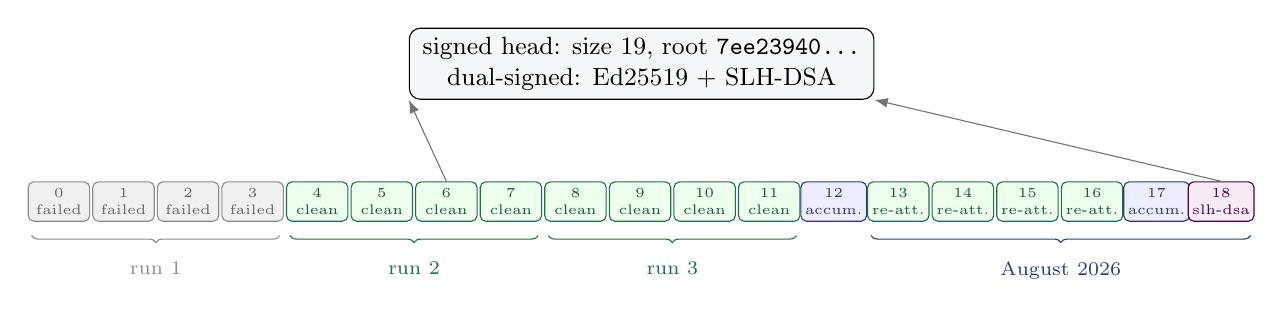
\begin{tikzpicture}[
  >=Latex,
  box/.style={draw,rounded corners=2pt,minimum width=.78cm,minimum height=.5cm,font=\tiny,align=center,inner sep=1.5pt},
  fail/.style={box,fill=black!6,draw=black!45,text=black!60},
  pq/.style={box,fill=violet!8,draw=violet!60!black,text=violet!55!black},
  ok/.style={box,fill=green!7!white,draw=deepgreen,text=deepgreen!80!black},
  acc/.style={box,fill=blue!7!white,draw=deepblue,text=deepblue},
  arrow/.style={->,draw=black!55}
]
\foreach \i in {0,...,3} {\node[fail] (l\i) at (0.82*\i,0) {\i\\failed};}
\foreach \i in {4,...,7} {\node[ok] (l\i) at (0.82*\i,0) {\i\\clean};}
\foreach \i in {8,...,11} {\node[ok] (l\i) at (0.82*\i,0) {\i\\clean};}
\node[acc] (l12) at (0.82*12,0) {12\\accum.};
\foreach \i in {13,...,16} {\node[ok] (l\i) at (0.82*\i,0) {\i\\re-att.};}
\node[acc] (l17) at (0.82*17,0) {17\\accum.};
\node[pq] (l18) at (0.82*18,0) {18\\slh-dsa};
\draw[decorate,decoration={brace,mirror,raise=5pt},black!45]
  ($(l0.south west)+(.05,0)$)--($(l3.south east)+(-.05,0)$)
  node[midway,below=11pt,font=\scriptsize]{run 1};
\draw[decorate,decoration={brace,mirror,raise=5pt},deepgreen]
  ($(l4.south west)+(.05,0)$)--($(l7.south east)+(-.05,0)$)
  node[midway,below=11pt,font=\scriptsize]{run 2};
\draw[decorate,decoration={brace,mirror,raise=5pt},deepgreen]
  ($(l8.south west)+(.05,0)$)--($(l11.south east)+(-.05,0)$)
  node[midway,below=11pt,font=\scriptsize]{run 3};
\draw[decorate,decoration={brace,mirror,raise=5pt},deepblue]
  ($(l13.south west)+(.05,0)$)--($(l18.south east)+(-.05,0)$)
  node[midway,below=11pt,font=\scriptsize]{August 2026};
\node[draw,rounded corners,fill=softgray,minimum width=5.9cm,minimum height=.85cm,align=center,font=\small] (sth) at (7.4,1.75)
  {signed head: size 19, root \code{7ee23940...}\\dual-signed: Ed25519 $+$ SLH-DSA};
\draw[arrow] (l6.north) -- (sth.south west);
\draw[arrow] (l18.north) -- (sth.south east);
\end{tikzpicture}
\caption{The public nineteen-leaf deployment. Failure leaves are retained; leaf
12 (the thirteenth entry) attests the accumulator corpus itself, scoped to the
recursive model; leaves 13--16 re-attest the four forks at 44 certificates
each; leaf 17 the hardened accumulator corpus; leaf 18 the SLH-DSA verify
path. Heads are dual-signed from size 14 on.}
\label{fig:deployment}
\end{figure}

\subsection{Mechanization coverage}

Leaf 12 is not a claim that the whole service is formally verified. The Lean
corpus covers the recursive Merkle model, inclusion completeness and
collision-extracting soundness, the consistency extractor, and the Merkle-layer
share of pin-store safety. The folklore whole-tree root-binding property (a root determines its
committed leaf list up to SHA-256 collision) is
mechanized through the specializations needed by the extractors rather than as
one quantified hash-fold theorem. Signature unforgeability, execution
provenance, the full signed-head state machine, asymptotic cost, and the
refinement from the deployed iterative consistency verifier remain outside the
corpus.

\begin{center}\small
\begin{tabularx}{\textwidth}{@{}l>{\raggedright\arraybackslash}X>{\raggedright\arraybackslash}X@{}}
\toprule
Layer & Mechanized evidence & Explicit boundary \\
\midrule
Merkle definitions & $\MTH$, $\Root$, $\Path$, recursive $\ConsRec$ & single SHA-256 boundary axiom \\
Inclusion & completeness and named collision extractor & collision resistance interpreted externally \\
Consistency & recursive-model soundness and extractor & no general consistency-completeness theorem \\
Pinning & per-step monotonicity and prefix correctness & signature layer and multi-step closure external \\
Deployment refinement & finite differential harness & no theorem for iterative verifier under authentic-pair invariant \\
Policy separation & deterministic tooling logic and regression tests & not mechanized in the leaf-12 corpus \\
Scheme-level games (\S\ref{sec:games}) & paper-level explicit reductions & two-transcript comparisons and prefix transport not mechanized \\
\bottomrule
\end{tabularx}
\end{center}

\subsection{Cost and reproducibility}

A replay of one Ed25519 fork requires approximately 30 minutes of end-to-end
resource-guarded (memory- and time-capped) replay time under the pinned environment, a figure corroborated by the
inter-leaf issuance spacing visible in the published log. Receipt verification requires one Ed25519
signature and a logarithmic number of SHA-256 node computations (the
complete inclusion core is printed as Appendix~\ref{app:verifier}). The
accumulator corpus is independently reviewable with a pinned public Lean
release; an environment-derived inventory fails closed on added, removed, or
axiom-smuggling declarations.

The fidelity harness compares the Lean-definition transliteration with the
deployed Python algorithms over pinned finite families:
\begin{center}\small
\begin{tabular}{@{}lrrl@{}}
\toprule
Family & Cases & Divergences & Interpretation \\
\midrule
Inclusion & 230,271 & 0 & baseline and out-of-range families \\
Consistency baseline & 230,016 & 0 & honest and mutation families \\
Lied-size consistency & 73,573 & 3,867 & all deployed-accepts-only \\
\bottomrule
\end{tabular}
\end{center}
Finite testing is not a proof of extensional equality. Here it served a more
valuable purpose: it falsified an overbroad equivalence claim and supplied a
stable regression boundary.

\begin{remark}[Model/deployment seam]
For malformed size claims, the deployed iterative verifier and the recursive
model are not extensionally equal (figures are the pre-closure measurement;
the $sn=0$ restoration reduces the divergence count in this family to zero).
In all 3,867 divergences observed across
the pinned families the deployed verifier accepted and the model rejected; the
reverse direction was not observed, and no global inclusion relation between
the two acceptance sets is claimed.
The public attestation therefore scopes soundness to the recursive model and
states the additional operational assumption: roots and sizes must be bound by
the authenticated pin-store and signed-head flow. This invariant is not
mechanized in the present corpus.
\end{remark}

\subsection{Consumer prototypes and version exactness}

The implemented internal consumer is a quorum-custody signing prototype: its
inbound boundary accepts a log-derived statement only when independently
attested verifier backends agree, and its policy consumes recorded
observations, never operator labels. Separately, an informal check found a
production codebase whose vendored Ed25519 dependency matches an attested
subject at family level but not at the attested version; the model treats a
family-level match as conferring nothing, because attestations are
version-exact by construction. Neither observation is an evaluation claim;
both indicate how the policy boundary is consumed in practice.

\subsection{Proof portability across forks}

Pure mathematical lemmas are largely reusable, while extraction-facing scripts
diverge where code structure and generated names diverge. In the deployed
corpora, the RISC~Zero and Betrusted signature-layer proof files differ by 27
changed lines (tracking one fork's optimization barrier and the forks'
differing operation order), other extraction-facing files differ by tens to
hundreds of lines, and pure carry and field lemmas remain byte-identical. This supports a practical conclusion: verification is portable
above the representation boundary and target-specific where implementation
structure actually differs.

\section{Related work}\label{sec:related}

\paragraph{Transparency.}
Certificate Transparency introduced publicly auditable append-only logs for
certificate issuance~\cite{ct1,ct2}; Crosby and Wallach built efficient
tamper-evident history trees~\cite{crosby}; Dowling et al. formalized security
notions for secure logging and CT~\cite{dghs} --- the games of
\S\ref{sec:games} adapt that two-transcript style to replay attestation, with
the operator as first-class adversary and policy separation as a deterministic
functionality. CONIKS applies transparency to
key directories~\cite{coniks}. LTL reuses the authenticated data structure but
changes the payload and trust semantics: a leaf is an observation of a proof
replay, not an issuance event or key binding.

\paragraph{Software supply-chain attestations.}
In-toto expresses supply-chain steps and link metadata~\cite{intoto}. Sigstore
combines ephemeral signing, identity, and transparency to reduce software-
signing adoption barriers~\cite{sigstore}. LTL is complementary: it concerns
what a theorem prover reportedly accepted and which assumptions remained, not
who built or signed a binary. A complete assurance chain should eventually
combine both.

\paragraph{Proof transport and verified cryptography.}
Proof-carrying code ships a proof to a consumer-side checker~\cite{pcc}. LTL
serves consumers that cannot deploy that checker and therefore accepts a
different trust trade. HACL*, EverCrypt, and Fiat-Crypto demonstrate verified
cryptographic implementation pipelines~\cite{hacl,evercrypt,fiatcrypto};
Computer-aided frameworks such as EasyCrypt address scheme-level security
proofs~\cite{easycrypt}; Aeneas targets functional verification of Rust
through translation~\cite{aeneas}.
LTL does not compete with those systems: it distributes accountable statements
about their replay.

\paragraph{Verification of transparency protocols.}
Cheval et al. mechanize transparency-protocol reasoning~\cite{cheval}.
The leaf-12 corpus approaches the composition from the opposite direction: it
mechanizes accumulator arguments and then logs that replay result. The
remaining refinement from the deployed state machine to the recursive model is
explicitly open.

\section{Limitations and research agenda}\label{sec:limitations}

The subject corpus maintains a numbered public file, \code{KNOWN-GAPS},
of fifteen gaps with their closure options (the scope block of
Appendix~\ref{app:entry13} cites its items 14 and 15); this section groups the load-bearing ones.

\paragraph{Operator observation trust.}
A malicious operator can fabricate a replay report. Signatures and Merkle
proofs make the lie attributable and persistent; they do not make it true.
Targeted independent replay is the corrective mechanism.

\paragraph{Replay-harness integrity.}
A wrong observation needs no malice: a defective replay harness --- a bug in
the audit driver, a fail-open guard, a truncated transcript --- produces the
same evidentiary damage as a dishonest operator, with the same accountability
answer (the record is attributable and persistent; independent replay corrects
it). The subject corpus's adversarial gate self-tests exist for exactly this
reason and reduce, but cannot eliminate, the exposure.

\paragraph{Theorem identity.}
Names and repository commits are not canonical semantic identifiers, and
commit identifiers are SHA-1-based --- a weaker binding than the log's own
SHA-256 tree. A future
schema should commit to elaborated theorem-type digests, axiom declaration-type
digests, and an environment or replay-manifest digest.

\paragraph{Source-to-binary gap.}
The evidence concerns source models at pinned commits. Reproducible builds,
compiler validation, binary measurement, and side-channel evidence are outside
the present result.

\paragraph{Witnessing and key distribution.}
The deployment has one operator and trust-on-first-use key distribution. A Git
mirror gives retaining observers a common public view, but does not force all
isolated clients to receive that view. Independent witnesses or gossip are the
natural next deployment step.

\paragraph{Consistency refinement.}
The recursive model is proved; the iterative deployment diverged from it on
malformed inputs, every observed divergence being deployed-accepts-only. The strongest closure is either to deploy
$\ConsRec$-equivalent semantics or to mechanize the signed-head and pin-store
flow and prove the authentic-pair refinement theorem.

\paragraph{Signed provenance.}
Signing-backend metadata is operator-provided context and should be committed
inside the signed tree-head payload. Even then it would remain an assertion,
not execution proof.

\paragraph{From accountable replay to cryptographic proof of replay.}
A longer-term direction is a succinct proof that a fixed proof-checker binary
accepted a fixed corpus. Such a system could reduce operator-observation trust,
but would introduce a new verified-execution stack. LTL supplies an
intermediate accountability layer and a public corpus against which that future
system can be evaluated.

\section{Conclusion}

Formal verification solves the production of correctness evidence; it does not
by itself solve distribution to consumers that cannot execute the verifier.
This paper isolates that second problem and gives a cryptographic answer based
on accountable replay attestation. The operator's observation remains trusted,
but its content is structured, its history is signed and append-only, its
assumption boundary is subject to consumer-local policy, and incompatible views
become attributable when compared.

The Lean Transparency Log demonstrates the complete construction. It amortizes
expensive replay over lightweight consumers, retains failed and superseded
observations, and carries a scoped attestation of the accumulator's own Lean
corpus as leaf 12. Just as importantly, the mechanization and differential
harness exposed a mismatch between the recursive model and the deployed
consistency verifier. Recording that mismatch in the public leaf is not a
failure of the method; it is evidence that the trust decomposition is doing
useful scientific work.

The next step is not to claim trustlessness. It is to close specific boundaries:
canonical theorem-type commitments, reproducible source-to-binary linkage,
independent witnesses, signed provenance commitments, and a proved refinement
between the deployed signed-head flow and the recursive model. Accountable
replay attestation provides an immediate infrastructure layer while those
stronger validity mechanisms are developed.

\section*{Artifact availability}
The live service is \url{https://ltl.zkdefi.org}. Leaf 12 (the log's thirteenth entry) has leaf hash
\begin{center}\small\ttfamily
8cb258d657f1fd00baaa9e0091e26c316cb69b591cb249a9543f51cade57c50a
\end{center}
and is included in the size-13 head with root
\begin{center}\small\ttfamily
3488a2d0ff9f00415bb561d61b01a420e3ca2e0f7b29351ec9ebb3f57319da0d
\end{center}
The public artifacts are available at:
\begin{itemize}[leftmargin=1.5em,itemsep=1pt]
\item append-only mirror: \href{https://github.com/saymrwulf/lean-transparency-log}{\texttt{saymrwulf/lean-transparency-log}};
\item accumulator mechanization: \href{https://github.com/saymrwulf/ltl-accumulator-verified}{\texttt{saymrwulf/ltl-accumulator-verified}};
\item provider and consumer tooling: \href{https://github.com/saymrwulf/proof-aware-crypto-tooling-agent}{\texttt{saymrwulf/proof-aware-crypto-tooling-agent}}.
\end{itemize}
A clone of the mirror re-verifies every numbered leaf, every published signed
head, and every published receipt offline via \code{python3 verify.py --all}
(Python standard library plus an \code{openssl} binary; the verifier fails
closed if signature checking is unavailable, and its adversarial self-test
ships beside it).

\section*{Acknowledgments}
The author designed the system and is responsible for every claim. Claude
(Anthropic) and GPT (OpenAI) were used as critical assistants in proof-corpus,
tooling, and manuscript review. Their output was not accepted as evidence;
claims were retained only after human review or reproducible artifact checks.

\begin{thebibliography}{23}
\itemsep2pt
\bibitem{ct1} B. Laurie, A. Langley, E. K\"asper. Certificate Transparency.
RFC 6962, 2013.

\bibitem{ct2} B. Laurie, E. Messeri, R. Stradling. Certificate Transparency
Version 2.0. RFC 9162, 2021.

\bibitem{crosby} S. A. Crosby, D. S. Wallach. Efficient Data Structures for
Tamper-Evident Logging. USENIX Security, pp. 317--334, 2009.

\bibitem{dghs} B. Dowling, F. G\"unther, U. Herath, D. Stebila. Secure
Logging Schemes and Certificate Transparency. ESORICS, LNCS 9879, pp.
140--158, 2016.

\bibitem{sigstore} Z. Newman, J. S. Meyers, S. Torres-Arias. Sigstore:
Software Signing for Everybody. ACM CCS, pp. 2353--2367, 2022.

\bibitem{intoto} S. Torres-Arias, H. Afzali, T. K. Kuppusamy, R. Curtmola,
J. Cappos. in-toto: Providing farm-to-table guarantees for bits and bytes.
USENIX Security, pp. 1393--1410, 2019.

\bibitem{coniks} M. S. Melara, A. Blankstein, J. Bonneau, E. W. Felten,
M. J. Freedman. CONIKS: Bringing Key Transparency to End Users. USENIX
Security, pp. 383--398, 2015.

\bibitem{pcc} G. C. Necula. Proof-Carrying Code. ACM POPL, pp. 106--119,
1997.

\bibitem{cheval} V. Cheval, J. Moreira, M. Ryan. Automatic verification of
transparency protocols. IEEE EuroS\&P, pp. 107--121, 2023.
doi:10.1109/EuroSP57164.2023.00016. arXiv:2303.04500.

\bibitem{easycrypt} G. Barthe, B. Gr\'egoire, S. Heraud, S. Zanella
B\'eguelin. Computer-Aided Security Proofs for the Working Cryptographer.
CRYPTO, LNCS 6841, pp. 71--90, 2011.

\bibitem{aeneas} S. Ho, J. Protzenko. Aeneas: Rust verification by
functional translation. Proc. ACM Program. Lang. 6 (ICFP): 711--741, 2022.

\bibitem{lean4} L. de Moura, S. Ullrich. The Lean 4 Theorem Prover and
Programming Language. CADE-28, LNCS 12699, pp. 625--635, 2021.

\bibitem{hacl} J.-K. Zinzindohou\'e, K. Bhargavan, J. Protzenko,
B. Beurdouche. HACL*: A Verified Modern Cryptographic Library. ACM CCS,
pp. 1789--1806, 2017.

\bibitem{evercrypt} J. Protzenko et al. EverCrypt: A Fast, Verified,
Cross-Platform Cryptographic Provider. IEEE S\&P, pp. 983--1002, 2020.

\bibitem{fiatcrypto} A. Erbsen, J. Philipoom, J. Gross, R. Sloan,
A. Chlipala. Simple High-Level Code for Cryptographic Arithmetic---With
Proofs, Without Compromises. IEEE S\&P, pp. 1202--1219, 2019.

\bibitem{eddsa} D. J. Bernstein, N. Duif, T. Lange, P. Schwabe, B.-Y. Yang.
High-speed high-security signatures. J. Cryptographic Engineering 2(2):
77--89, 2012.

\bibitem{rfc8032} S. Josefsson, I. Liusvaara. Edwards-Curve Digital
Signature Algorithm (EdDSA). RFC 8032, 2017.

\bibitem{edwards} D. J. Bernstein, T. Lange. Faster addition and doubling on
elliptic curves. ASIACRYPT, LNCS 4833, pp. 29--50, 2007.

\bibitem{twisted} D. J. Bernstein, P. Birkner, M. Joye, T. Lange,
C. Peters. Twisted Edwards curves. AFRICACRYPT, LNCS 5023, pp. 389--405,
2008.

\bibitem{pnueli} A. Pnueli. The temporal logic of programs. IEEE FOCS, pp.
46--57, 1977.


\bibitem{rogaway} P. Rogaway. Formalizing Human Ignorance:
Collision-Resistant Hashing without the Keys. VIETCRYPT, LNCS 4341, pp.
211--228, 2006. doi:10.1007/11958239\_14.

\bibitem{klaus2026} N. Klaus, J. Conejero, P. Tolmach. A Rust-to-Lean
Verification Pipeline with AI Provers: An Experience Report. arXiv:2605.30106,
2026.

\bibitem{fips205} National Institute of Standards and Technology.
Stateless Hash-Based Digital Signature Standard. FIPS 205, August 2024.

\end{thebibliography}

% Appendix policy (declared 2026-08-16): the appendix block starts on a
% fresh page and then flows continuously -- no page breaks between
% individual appendices. The claim matrix is one unbreakable tabularx.
\clearpage
\appendix

\section{End-to-end claim matrix}\label{app:matrix}
\begin{center}\small
\begin{tabularx}{\textwidth}{@{}>{\raggedright\arraybackslash}X>{\raggedright\arraybackslash}X>{\raggedright\arraybackslash}X@{}}
\toprule
Consumer conclusion & Established by & Remaining assumption \\
\midrule
Leaf has an authentic opening with a position-bound leaf value at index $m$ under head $h$ & inclusion proof and signed head & \mbox{SHA-256} collision resistance; correct public key; \mbox{EUF-CMA} of the head signature \\
\addlinespace[3pt]
Head root commits the published numbered leaf list & full-mirror recomputation (\code{verify.py --all}) & mirror availability and retention \\
\addlinespace[3pt]
Head was authorized by the log identity & Ed25519 verification & correct key acquisition; \mbox{EUF-CMA} \\
\addlinespace[3pt]
New pinned head extends old pinned head & consistency proof & \mbox{SHA-256} collision resistance; recursive-model soundness; authentic size/root pairing for deployment \\
\addlinespace[3pt]
Equal-size unequal roots in one log context conflict & two valid signatures & correct public key; \mbox{EUF-CMA}; operationally, a retaining observer must compare the heads \\
\addlinespace[3pt]
Observed cone matches local boundary policy & exact set equality & semantic identity of named declarations \\
\addlinespace[3pt]
Operator claims the kernel produced the observation & attestation signature and leaf inclusion & correct provider key; \mbox{EUF-CMA} \\
\addlinespace[3pt]
Kernel actually produced the recorded observation & not cryptographically established; independently checkable by replay & operator and replay-pipeline honesty, or faithful independent replay \\
\addlinespace[3pt]
Recorded cone was produced by an audit that performed its checks & not established --- the audit driver is itself part of the replay pipeline & audit-gate integrity; adversarial gate self-tests reduce this exposure, they do not eliminate it \\
\addlinespace[3pt]
Source corresponds to deployed binary & not established & reproducible build and compiler assurance \\
\addlinespace[3pt]
Claimed signer implementation produced STH & not established & execution provenance \\
\bottomrule
\end{tabularx}
\end{center}

\section{Deployed leaf-12 scope}\label{app:entry13}
Leaf 12 contains the following deployment constraint,
quoted verbatim, in its machine-readable scope block:
\begin{quote}\small
Attestation scope: this corpus kernel-checks the listed theorems about the
mechanized recursive accumulator model. Correspondence with the deployed
inclusion verifier is supported by finite differential testing over the pinned
families. The deployed consistency verifier is not extensionally equal to the
model; applying the mechanized soundness result to the deployed consumer flow
additionally relies on an unmechanized authentic-size/root invariant
(KNOWN-GAPS 14/15).
\end{quote}
Its exclusions name SHA-256 collision resistance, deployed-verifier extensional
equality, the signature/STH layer, and asymptotic cost claims.

\section{Compact receipt-verification core}\label{app:verifier}
The following code is only the Merkle inclusion core. A complete receipt
verifier must additionally validate the signed tree head, log identifier,
tree-size binding, public-key fingerprint or pinned key, leaf hash, and receipt
schema. The published log-repository verifier implements that full binding
list for every published receipt --- the binding fields are required, never
compare-if-present --- and fails closed when signature checking is
unavailable.
\begin{lstlisting}[language=Python]
import hashlib

def H(data):
    return hashlib.sha256(data).digest()

def h_leaf(data):
    return H(b"\x00" + data)

def h_node(left, right):
    return H(b"\x01" + left + right)

def split_below(n):
    return 1 << ((n - 1).bit_length() - 1)

def take(path, used):
    if used >= len(path):
        raise ValueError("proof exhausted")
    return path[used]

def root(value, index, size, path, used=0):
    if size == 1:
        return value, used
    k = split_below(size)
    if index < k:
        left, used = root(value, index, k, path, used)
        return h_node(left, take(path, used)), used + 1
    right, used = root(value, index-k, size-k, path, used)
    return h_node(take(path, used), right), used + 1

def verify_inclusion(leaf, index, size, path, expected_root):
    if size <= 0 or index < 0 or index >= size:
        return False
    try:
        result, used = root(h_leaf(leaf), index, size, path)
    except ValueError:
        return False
    return used == len(path) and result == expected_root
\end{lstlisting}

\section{Four Ed25519 verification tiers}\label{app:tiers}
\begin{center}\small
\begin{tabular}{@{}lll@{}}
\toprule
Tier & Meaning & Upstream Lean declaration \\
\midrule
T1 & byte-level acceptance equation & \code{verify_accepts_iff} \\
T2 & canonical encoding lift & \code{verify_accepts_iff_point} \\
T3 & injectivity / point equation & \code{verify_accepts_iff_point_eq} \\
T4 & constructive decompression lift & \code{verify_accepts_iff_decompress} \\
\bottomrule
\end{tabular}
\end{center}

All four tiers share one opaque boundary --- the SHA-512 challenge hash
and the selected wire-format interfaces (\S\ref{sec:instantiation});
the arithmetic and group certificates beneath them rest on Lean's
foundational axioms alone.

\section{SLH-DSA verification certificates and their cones}\label{app:slhtiers}

Eleven certificates over the extracted SLH-DSA-SHA2-128s verify path
(leaf 18). Beyond Lean's three foundational axioms, each certificate's
exact axiom set consists of the uninterpreted hash oracles listed ---
enforced by the audit as set equality in both directions, so the table is
machine-checked, not documentation. The cone grows with the layer: pure
digit/byte arithmetic rests on the kernel alone; the apex carries all
five oracles.

\begin{center}\small
\begin{tabular}{@{}lll@{}}
\toprule
Layer & Lean declaration(s) & Oracles in the cone \\
\midrule
Digit/byte plumbing & \code{to_int_loop_eq}, \code{to_byte_loop_eq} & --- \\
 & \code{wots_csum_loop_eq}, \code{base2b_outer_loop_eq} & \\
Chain walk & \code{chain_free_loop_eq} & \code{f} \\
WOTS pk recomputation & \code{wots_loop1_eq} & \code{f} \\
XMSS Merkle ascent & \code{xmss_loop_eq} & \code{h} \\
FORS inner ascent & \code{fors_inner_loop_eq} & \code{h} \\
FORS outer loop & \code{fors_outer_loop_eq} & \code{f}, \code{h} \\
Hypertree walk & \code{ht_loop_eq} & \code{f}, \code{h}, \code{t_l} \\
Acceptance characterization & \code{slh_verify_128s_accepts_iff} & all five \\
\bottomrule
\end{tabular}
\end{center}

The oracles model the parameter set's SHA-256 hash-suite instantiations:
\code{h_msg} (message digest), \code{f} (chain step and FORS leaf),
\code{h} (Merkle node), \code{t_l} and \code{t_len} (the WOTS and FORS
compressors --- two axioms over what is one Rust primitive, deliberately
conservative, with the source's naming inversion against the standard's
$T_\ell$/$T_k$ documented at the declarations). The acceptance characterization is proved directly from the verifier's
structure, not by composing the ten loop theorems --- it would remain
provable if any of the ten were deleted. Conversely, each loop
certificate carries assurance only insofar as a human has checked its
reference fold against the corresponding FIPS~205 algorithm.

\end{document}
